\begin{exercise}
      {ID-a6852151fc20fd2fdb5d2cbeb651d19974598f9b}
      {Die Quadratur des Kreuzes}
  \ifproblem\problem
    Zerschneide das Kreuz so, dass du aus den Teilen ein Quadrat mit demselben
    Flächeninhalt legen kannst.
    \begin{center}
      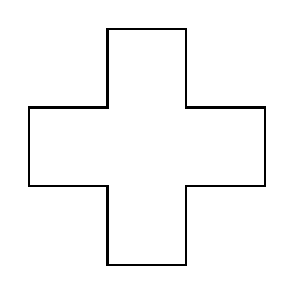
\begin{tikzpicture}[scale=0.5]
        \draw[line width=0.8pt]
              ( 1,  1) --
              ( 1,  3) --
              (-1,  3) --
              (-1,  1) --
              (-3,  1) --
              (-3, -1) --
              (-1, -1) --
              (-1, -3) --
              ( 1, -3) --
              ( 1, -1) --
              ( 3, -1) --
              ( 3,  1) -- cycle;
      \end{tikzpicture}
    \end{center}
  \fi
  %\ifoutline\outline
  %\fi
  %\ifoutcome\outcome
  %\fi
\end{exercise}
